\chapter{Pocesso}

Para a verificação deste documento foi elaborado o processo da figura~\ref{fig:processo}.


\begin{figure}[H]
  \center
  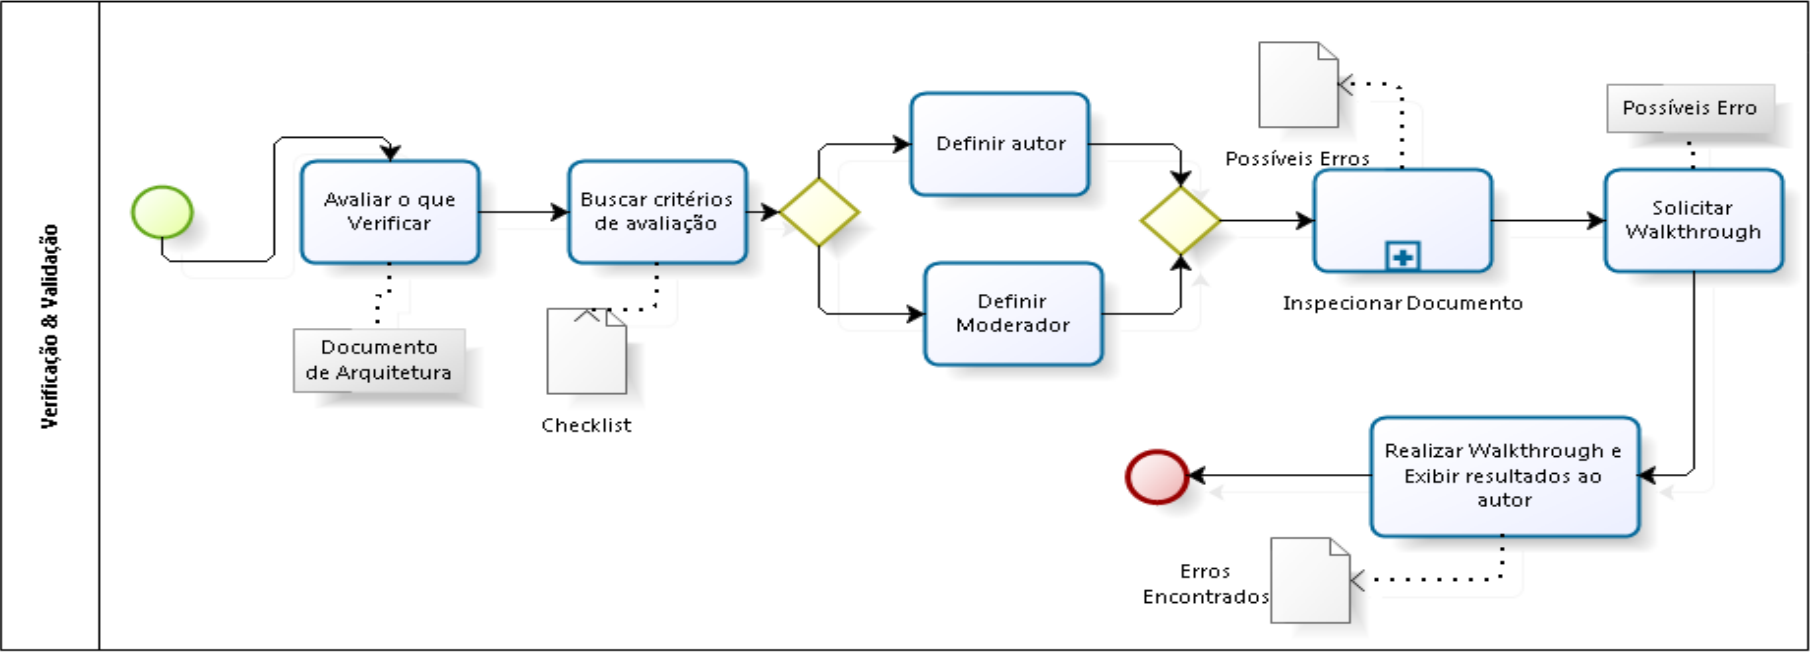
\includegraphics[width=1\textwidth]{figuras/processo.png}
  \caption{Processo}
  \label{fig:processo}
\end{figure}

\section{Avaliar o que Verificar}

Escolher qual documento seria inspecionado. Definido de acordo com o que foi dito nos parágrafos anteriores. 

\section{Buscar Critérios}

Definir quais elementos seriam inspecionados e com base em quais critérios. 

    \subsection{Check list}
    Foi definido um checklist com os critérios escolhidos de acordo com o template oferecido no site \url{http://www.funpar.ufpr.br:8080/rup/webtmpl/templates/a_and_d/rup_sad.html} o qual define tópicos obrigatórios na construção do documento de arquitetura. Os tópicos são: 

    \begin{itemize}
        \item Introdução
            \begin{itemize}
                \item Finalidade     
                \item Escopo     
                \item Definições, Acrônimos e Abreviações     
                \item Referências     
                \item Visão Geral
            \end{itemize}
        \item Representação de arquitetura
        \item Metas e Restrições de Arquitetura
        \item Visão de Caso de Uso 
            \begin{itemize}
                \item Realização de Casos de Uso
            \end{itemize}
        \item Visão Lógica
    \end{itemize}

    Os pontos de avaliação, com base em outras referências~\cite{stafford2004creating}\cite{clements2002documenting} são os da figura~\ref{fig:criterios}.

\begin{figure}[H]
  \center
  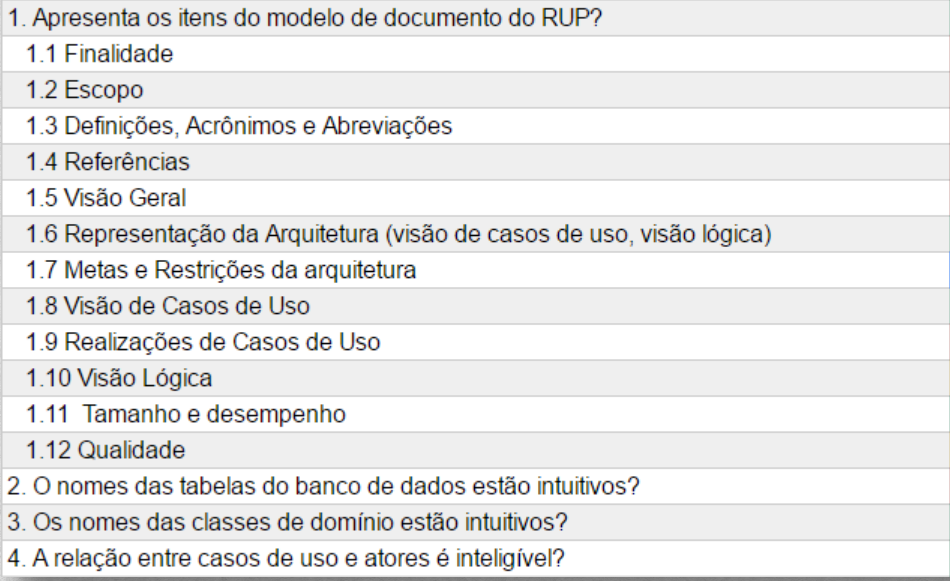
\includegraphics[width=1\textwidth]{figuras/criterios.png}
  \caption{Criterios}
  \label{fig:criterios}
\end{figure}

\section{Definir Autor}

 Identificar o autor do documento escolhido. 

 \subsection{Grupo do Sushizuki}

 O documento escolhido para verificação foi o de Arquitetura do projeto Sushizuki, disponível em \url{https://github.com/sushizuki/main-project/wiki/Documento-de-Arquitetura} , desenvolvido para a matéria de Desenho de Software ofertada na Universidade de Brasília campus Gama.


 \section{Definir Moderador}

 Identificar os autores da inspeção e seus papeis. 

 \subsection{-----}

 \section{Inspecionar Documento}

 \subsection{Checklist}

 \section{Solicitar e Realizar Walkthrough}

 \subsection{----}

 \section{Resultados}

 Entregar o resultado da inspeção para o autor 

\begin{figure}[H]
  \center
  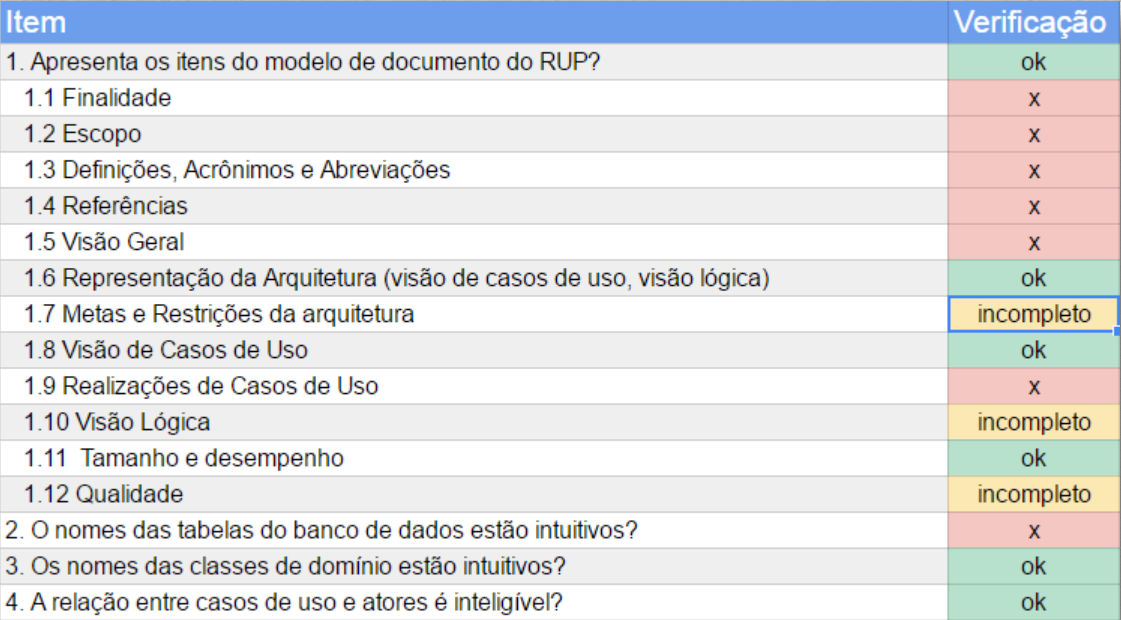
\includegraphics[width=1\textwidth]{figuras/checklist-results.png}
  \caption{Resultados Checklist}
  \label{fig:checklist-results}
\end{figure}

 \subsection{}
